\documentclass[twoside]{book}

% Packages required by doxygen
\usepackage{fixltx2e}
\usepackage{calc}
\usepackage{doxygen}
\usepackage[export]{adjustbox} % also loads graphicx
\usepackage{graphicx}
\usepackage[utf8]{inputenc}
\usepackage{makeidx}
\usepackage{multicol}
\usepackage{multirow}
\PassOptionsToPackage{warn}{textcomp}
\usepackage{textcomp}
\usepackage[nointegrals]{wasysym}
\usepackage[table]{xcolor}

% Font selection
\usepackage[T1]{fontenc}
\usepackage[scaled=.90]{helvet}
\usepackage{courier}
\usepackage{amssymb}
\usepackage{sectsty}
\renewcommand{\familydefault}{\sfdefault}
\allsectionsfont{%
  \fontseries{bc}\selectfont%
  \color{darkgray}%
}
\renewcommand{\DoxyLabelFont}{%
  \fontseries{bc}\selectfont%
  \color{darkgray}%
}
\newcommand{\+}{\discretionary{\mbox{\scriptsize$\hookleftarrow$}}{}{}}

% Page & text layout
\usepackage{geometry}
\geometry{%
  a4paper,%
  top=2.5cm,%
  bottom=2.5cm,%
  left=2.5cm,%
  right=2.5cm%
}
\tolerance=750
\hfuzz=15pt
\hbadness=750
\setlength{\emergencystretch}{15pt}
\setlength{\parindent}{0cm}
\setlength{\parskip}{3ex plus 2ex minus 2ex}
\makeatletter
\renewcommand{\paragraph}{%
  \@startsection{paragraph}{4}{0ex}{-1.0ex}{1.0ex}{%
    \normalfont\normalsize\bfseries\SS@parafont%
  }%
}
\renewcommand{\subparagraph}{%
  \@startsection{subparagraph}{5}{0ex}{-1.0ex}{1.0ex}{%
    \normalfont\normalsize\bfseries\SS@subparafont%
  }%
}
\makeatother

% Headers & footers
\usepackage{fancyhdr}
\pagestyle{fancyplain}
\fancyhead[LE]{\fancyplain{}{\bfseries\thepage}}
\fancyhead[CE]{\fancyplain{}{}}
\fancyhead[RE]{\fancyplain{}{\bfseries\leftmark}}
\fancyhead[LO]{\fancyplain{}{\bfseries\rightmark}}
\fancyhead[CO]{\fancyplain{}{}}
\fancyhead[RO]{\fancyplain{}{\bfseries\thepage}}
\fancyfoot[LE]{\fancyplain{}{}}
\fancyfoot[CE]{\fancyplain{}{}}
\fancyfoot[RE]{\fancyplain{}{\bfseries\scriptsize Generated by Doxygen }}
\fancyfoot[LO]{\fancyplain{}{\bfseries\scriptsize Generated by Doxygen }}
\fancyfoot[CO]{\fancyplain{}{}}
\fancyfoot[RO]{\fancyplain{}{}}
\renewcommand{\footrulewidth}{0.4pt}
\renewcommand{\chaptermark}[1]{%
  \markboth{#1}{}%
}
\renewcommand{\sectionmark}[1]{%
  \markright{\thesection\ #1}%
}

% Indices & bibliography
\usepackage{natbib}
\usepackage[titles]{tocloft}
\setcounter{tocdepth}{3}
\setcounter{secnumdepth}{5}
\makeindex

% Hyperlinks (required, but should be loaded last)
\usepackage{ifpdf}
\ifpdf
  \usepackage[pdftex,pagebackref=true]{hyperref}
\else
  \usepackage[ps2pdf,pagebackref=true]{hyperref}
\fi
\hypersetup{%
  colorlinks=true,%
  linkcolor=blue,%
  citecolor=blue,%
  unicode%
}

% Custom commands
\newcommand{\clearemptydoublepage}{%
  \newpage{\pagestyle{empty}\cleardoublepage}%
}

\usepackage{caption}
\captionsetup{labelsep=space,justification=centering,font={bf},singlelinecheck=off,skip=4pt,position=top}

%===== C O N T E N T S =====

\begin{document}

% Titlepage & ToC
\hypersetup{pageanchor=false,
             bookmarksnumbered=true,
             pdfencoding=unicode
            }
\pagenumbering{roman}
\begin{titlepage}
\vspace*{7cm}
\begin{center}%
{\Large robot\+\_\+properties\+\_\+teststand }\\
\vspace*{1cm}
{\large Generated by Doxygen 1.8.11}\\
\end{center}
\end{titlepage}
\clearemptydoublepage
\tableofcontents
\clearemptydoublepage
\pagenumbering{arabic}
\hypersetup{pageanchor=true}

%--- Begin generated contents ---
\chapter{robot\+\_\+properties\+\_\+teststand}
\label{md_readme}
\hypertarget{md_readme}{}
\subsection*{What is it}

This package is a collection of tools offen used in C++ such as clipping data, ...

\subsection*{Authors}

Manuel Wuthrich

\subsection*{Copyrights}

Copyright (c) 2019, New York University and Max Planck Gesellschaft.

\subsection*{License}

License B\+S\+D-\/3-\/\+Clause 
\chapter{License}
\label{license}
\hypertarget{license}{}

\begin{DoxyRefList}
\item[\label{license__license000001}%
\hypertarget{license__license000001}{}%
File \hyperlink{AtiFTSensor_8h}{Ati\+F\+T\+Sensor.h} ]License B\+S\+D-\/3-\/\+Clause 
\end{DoxyRefList}
\chapter{Namespace Index}
\section{Namespace List}
Here is a list of all documented namespaces with brief descriptions\+:\begin{DoxyCompactList}
\item\contentsline{section}{\hyperlink{namespaceblmc__drivers}{blmc\+\_\+drivers} \\*This namespace is the standard namespace of the package }{\pageref{namespaceblmc__drivers}}{}
\item\contentsline{section}{\hyperlink{namespaceosi}{osi} \\*Common include }{\pageref{namespaceosi}}{}
\end{DoxyCompactList}

\chapter{Hierarchical Index}
\section{Class Hierarchy}
This inheritance list is sorted roughly, but not completely, alphabetically\+:\begin{DoxyCompactList}
\item \contentsline{section}{py\+\_\+robot\+\_\+properties\+\_\+teststand.\+config.\+Teststand\+Config}{\pageref{classpy__robot__properties__teststand_1_1config_1_1TeststandConfig}}{}
\item Pin\+Bullet\+Wrapper\begin{DoxyCompactList}
\item \contentsline{section}{py\+\_\+robot\+\_\+properties\+\_\+teststand.\+teststand\+\_\+wrapper.\+Teststand\+Robot}{\pageref{classpy__robot__properties__teststand_1_1teststand__wrapper_1_1TeststandRobot}}{}
\end{DoxyCompactList}
\end{DoxyCompactList}

\chapter{Class Index}
\section{Class List}
Here are the classes, structs, unions and interfaces with brief descriptions\+:\begin{DoxyCompactList}
\item\contentsline{section}{\hyperlink{classmct_1_1LinearDynamics}{mct\+::\+Linear\+Dynamics} }{\pageref{classmct_1_1LinearDynamics}}{}
\item\contentsline{section}{\hyperlink{classmct_1_1LinearDynamicsWithAccelerationConstraint}{mct\+::\+Linear\+Dynamics\+With\+Acceleration\+Constraint} }{\pageref{classmct_1_1LinearDynamicsWithAccelerationConstraint}}{}
\item\contentsline{section}{\hyperlink{classmct_1_1NonnegDouble}{mct\+::\+Nonneg\+Double} }{\pageref{classmct_1_1NonnegDouble}}{}
\item\contentsline{section}{\hyperlink{classmct_1_1SafetyConstraint}{mct\+::\+Safety\+Constraint} }{\pageref{classmct_1_1SafetyConstraint}}{}
\end{DoxyCompactList}

\chapter{File Index}
\section{File List}
Here is a list of all documented files with brief descriptions\+:\begin{DoxyCompactList}
\item\contentsline{section}{demos/\hyperlink{const__torque__control_8cpp}{const\+\_\+torque\+\_\+control.\+cpp} }{\pageref{const__torque__control_8cpp}}{}
\item\contentsline{section}{demos/\hyperlink{const__torque__control_8hpp}{const\+\_\+torque\+\_\+control.\+hpp} }{\pageref{const__torque__control_8hpp}}{}
\item\contentsline{section}{demos/\hyperlink{demo__1__motor_8cpp}{demo\+\_\+1\+\_\+motor.\+cpp} }{\pageref{demo__1__motor_8cpp}}{}
\item\contentsline{section}{demos/\hyperlink{demo__1__motor__print__everything_8cpp}{demo\+\_\+1\+\_\+motor\+\_\+print\+\_\+everything.\+cpp} }{\pageref{demo__1__motor__print__everything_8cpp}}{}
\item\contentsline{section}{demos/\hyperlink{demo__2__motors_8cpp}{demo\+\_\+2\+\_\+motors.\+cpp} }{\pageref{demo__2__motors_8cpp}}{}
\item\contentsline{section}{demos/\hyperlink{demo__3__motors_8cpp}{demo\+\_\+3\+\_\+motors.\+cpp} }{\pageref{demo__3__motors_8cpp}}{}
\item\contentsline{section}{demos/\hyperlink{demo__8__motors_8cpp}{demo\+\_\+8\+\_\+motors.\+cpp} }{\pageref{demo__8__motors_8cpp}}{}
\item\contentsline{section}{demos/\hyperlink{demo__const__torque__1__motor_8cpp}{demo\+\_\+const\+\_\+torque\+\_\+1\+\_\+motor.\+cpp} }{\pageref{demo__const__torque__1__motor_8cpp}}{}
\item\contentsline{section}{demos/\hyperlink{demo__ethernet_8cpp}{demo\+\_\+ethernet.\+cpp} }{\pageref{demo__ethernet_8cpp}}{}
\item\contentsline{section}{demos/\hyperlink{demo__leg_8cpp}{demo\+\_\+leg.\+cpp} }{\pageref{demo__leg_8cpp}}{}
\item\contentsline{section}{demos/\hyperlink{demo__sine__position__1__motor_8cpp}{demo\+\_\+sine\+\_\+position\+\_\+1\+\_\+motor.\+cpp} }{\pageref{demo__sine__position__1__motor_8cpp}}{}
\item\contentsline{section}{demos/\hyperlink{demo__sine__torque__1__motor_8cpp}{demo\+\_\+sine\+\_\+torque\+\_\+1\+\_\+motor.\+cpp} }{\pageref{demo__sine__torque__1__motor_8cpp}}{}
\item\contentsline{section}{demos/\hyperlink{demo__single__board_8cpp}{demo\+\_\+single\+\_\+board.\+cpp} }{\pageref{demo__single__board_8cpp}}{}
\item\contentsline{section}{demos/\hyperlink{pd__control_8cpp}{pd\+\_\+control.\+cpp} }{\pageref{pd__control_8cpp}}{}
\item\contentsline{section}{demos/\hyperlink{pd__control_8hpp}{pd\+\_\+control.\+hpp} }{\pageref{pd__control_8hpp}}{}
\item\contentsline{section}{demos/\hyperlink{sine__position__control_8cpp}{sine\+\_\+position\+\_\+control.\+cpp} }{\pageref{sine__position__control_8cpp}}{}
\item\contentsline{section}{demos/\hyperlink{sine__position__control_8hpp}{sine\+\_\+position\+\_\+control.\+hpp} }{\pageref{sine__position__control_8hpp}}{}
\item\contentsline{section}{demos/\hyperlink{sine__torque__control_8cpp}{sine\+\_\+torque\+\_\+control.\+cpp} }{\pageref{sine__torque__control_8cpp}}{}
\item\contentsline{section}{demos/\hyperlink{sine__torque__control_8hpp}{sine\+\_\+torque\+\_\+control.\+hpp} }{\pageref{sine__torque__control_8hpp}}{}
\item\contentsline{section}{include/blmc\+\_\+drivers/\hyperlink{serial__reader_8hpp}{serial\+\_\+reader.\+hpp} \\*Wrapper for reading new-\/line terminated list of values from serial port }{\pageref{serial__reader_8hpp}}{}
\item\contentsline{section}{include/blmc\+\_\+drivers/devices/\hyperlink{analog__sensor_8hpp}{analog\+\_\+sensor.\+hpp} }{\pageref{analog__sensor_8hpp}}{}
\item\contentsline{section}{include/blmc\+\_\+drivers/devices/\hyperlink{can__bus_8hpp}{can\+\_\+bus.\+hpp} }{\pageref{can__bus_8hpp}}{}
\item\contentsline{section}{include/blmc\+\_\+drivers/devices/\hyperlink{device__interface_8hpp}{device\+\_\+interface.\+hpp} }{\pageref{device__interface_8hpp}}{}
\item\contentsline{section}{include/blmc\+\_\+drivers/devices/\hyperlink{leg_8hpp}{leg.\+hpp} }{\pageref{leg_8hpp}}{}
\item\contentsline{section}{include/blmc\+\_\+drivers/devices/\hyperlink{motor_8hpp}{motor.\+hpp} }{\pageref{motor_8hpp}}{}
\item\contentsline{section}{include/blmc\+\_\+drivers/devices/\hyperlink{motor__board_8hpp}{motor\+\_\+board.\+hpp} }{\pageref{motor__board_8hpp}}{}
\item\contentsline{section}{include/blmc\+\_\+drivers/devices/\hyperlink{spi__bus_8hpp}{spi\+\_\+bus.\+hpp} \\*Interface for the main board designed by Thomas Floyols \href{https://github.com/open-dynamic-robot-initiative/master-board}{\tt https\+://github.\+com/open-\/dynamic-\/robot-\/initiative/master-\/board} }{\pageref{spi__bus_8hpp}}{}
\item\contentsline{section}{include/blmc\+\_\+drivers/devices/\hyperlink{spi__motor__board_8hpp}{spi\+\_\+motor\+\_\+board.\+hpp} \\*Interface for the master board designed by Thomas Floyols \href{https://github.com/open-dynamic-robot-initiative/master-board}{\tt https\+://github.\+com/open-\/dynamic-\/robot-\/initiative/master-\/board} }{\pageref{spi__motor__board_8hpp}}{}
\item\contentsline{section}{include/blmc\+\_\+drivers/utils/\hyperlink{os__interface_8hpp}{os\+\_\+interface.\+hpp} }{\pageref{os__interface_8hpp}}{}
\item\contentsline{section}{src/\hyperlink{analog__sensors_8cpp}{analog\+\_\+sensors.\+cpp} \\*This file defines a class to get access to analogue sensors }{\pageref{analog__sensors_8cpp}}{}
\item\contentsline{section}{src/\hyperlink{can__bus_8cpp}{can\+\_\+bus.\+cpp} \\*This file defines classes that allow communication with a Can network }{\pageref{can__bus_8cpp}}{}
\item\contentsline{section}{src/\hyperlink{motor_8cpp}{motor.\+cpp} }{\pageref{motor_8cpp}}{}
\item\contentsline{section}{src/\hyperlink{motor__board_8cpp}{motor\+\_\+board.\+cpp} \\*This file implements the classes from \char`\"{}blmc\+\_\+drivers/devices/motor\+\_\+board.\+hpp\char`\"{} }{\pageref{motor__board_8cpp}}{}
\item\contentsline{section}{src/\hyperlink{serial__reader_8cpp}{serial\+\_\+reader.\+cpp} \\*Wrapper for reading new-\/line terminated list of values from serial port }{\pageref{serial__reader_8cpp}}{}
\item\contentsline{section}{src/\hyperlink{spi__bus_8cpp}{spi\+\_\+bus.\+cpp} \\*This file implements the classes from \char`\"{}blmc\+\_\+drivers/devices/motor\+\_\+board.\+hpp\char`\"{} }{\pageref{spi__bus_8cpp}}{}
\item\contentsline{section}{src/\hyperlink{spi__motor__board_8cpp}{spi\+\_\+motor\+\_\+board.\+cpp} \\*This file implements the classes from \char`\"{}blmc\+\_\+drivers/devices/motor\+\_\+board.\+hpp\char`\"{} }{\pageref{spi__motor__board_8cpp}}{}
\end{DoxyCompactList}

\chapter{Namespace Documentation}
\hypertarget{namespacepy__robot__properties__teststand}{}\section{py\+\_\+robot\+\_\+properties\+\_\+teststand Namespace Reference}
\label{namespacepy__robot__properties__teststand}\index{py\+\_\+robot\+\_\+properties\+\_\+teststand@{py\+\_\+robot\+\_\+properties\+\_\+teststand}}


Define the python interface of the robot model using pinocchio and python.  




\subsection{Detailed Description}
Define the python interface of the robot model using pinocchio and python. 

\begin{DoxyAuthor}{Author}
Maximilien Naveau (\href{mailto:maximilien.naveau@gmail.com}{\tt maximilien.\+naveau@gmail.\+com}) 
\end{DoxyAuthor}
\begin{DoxyRefDesc}{License}
\item[\hyperlink{license__license000002}{License}]License B\+S\+D-\/3-\/\+Clause \end{DoxyRefDesc}
\begin{DoxyCopyright}{Copyright}
Copyright (c) 2019, New York University and Max Planck Gesellschaft. 
\end{DoxyCopyright}
\begin{DoxyDate}{Date}
2019-\/05-\/22 
\end{DoxyDate}

\chapter{Class Documentation}
\hypertarget{classpy__robot__properties__teststand_1_1config_1_1TeststandConfig}{}\section{py\+\_\+robot\+\_\+properties\+\_\+teststand.\+config.\+Teststand\+Config Class Reference}
\label{classpy__robot__properties__teststand_1_1config_1_1TeststandConfig}\index{py\+\_\+robot\+\_\+properties\+\_\+teststand.\+config.\+Teststand\+Config@{py\+\_\+robot\+\_\+properties\+\_\+teststand.\+config.\+Teststand\+Config}}
\subsection*{Public Member Functions}
\begin{DoxyCompactItemize}
\item 
def {\bfseries build\+Robot\+Wrapper} (cls)\hypertarget{classpy__robot__properties__teststand_1_1config_1_1TeststandConfig_ad0bd7dd74ddf8ca9f8a4c8523f560e6e}{}\label{classpy__robot__properties__teststand_1_1config_1_1TeststandConfig_ad0bd7dd74ddf8ca9f8a4c8523f560e6e}

\end{DoxyCompactItemize}
\subsection*{Static Public Attributes}
\begin{DoxyCompactItemize}
\item 
string {\bfseries robot\+\_\+name} = \char`\"{}teststand\char`\"{}\hypertarget{classpy__robot__properties__teststand_1_1config_1_1TeststandConfig_ab68e64f324ea47a4c81f9cc82aeb6cf4}{}\label{classpy__robot__properties__teststand_1_1config_1_1TeststandConfig_ab68e64f324ea47a4c81f9cc82aeb6cf4}

\item 
float {\bfseries kp} = 5.\+0\hypertarget{classpy__robot__properties__teststand_1_1config_1_1TeststandConfig_a360b8c5b84b6849da15236a2c98ff991}{}\label{classpy__robot__properties__teststand_1_1config_1_1TeststandConfig_a360b8c5b84b6849da15236a2c98ff991}

\item 
float {\bfseries kd} = 0.\+1\hypertarget{classpy__robot__properties__teststand_1_1config_1_1TeststandConfig_ac8ef3cbf2ca5a3b84dac6713cfab2a90}{}\label{classpy__robot__properties__teststand_1_1config_1_1TeststandConfig_ac8ef3cbf2ca5a3b84dac6713cfab2a90}

\item 
float {\bfseries ki} = 0.\+0\hypertarget{classpy__robot__properties__teststand_1_1config_1_1TeststandConfig_a1beb333b141d33d055368ff5418b3c09}{}\label{classpy__robot__properties__teststand_1_1config_1_1TeststandConfig_a1beb333b141d33d055368ff5418b3c09}

\item 
tuple {\bfseries urdf\+\_\+path}
\item 
list {\bfseries meshes\+\_\+path}
\item 
tuple {\bfseries yaml\+\_\+path}
\item 
float {\bfseries motor\+\_\+inertia} = 0.\+0000045\hypertarget{classpy__robot__properties__teststand_1_1config_1_1TeststandConfig_a0d2f901b065d005500004294a0999ed7}{}\label{classpy__robot__properties__teststand_1_1config_1_1TeststandConfig_a0d2f901b065d005500004294a0999ed7}

\item 
int {\bfseries motor\+\_\+gear\+\_\+ration} = 9\hypertarget{classpy__robot__properties__teststand_1_1config_1_1TeststandConfig_a934b88c4ed3899692dafb89134bfe3da}{}\label{classpy__robot__properties__teststand_1_1config_1_1TeststandConfig_a934b88c4ed3899692dafb89134bfe3da}

\item 
float {\bfseries motor\+\_\+torque\+\_\+constant} = 0.\+025\hypertarget{classpy__robot__properties__teststand_1_1config_1_1TeststandConfig_afac43884ea08cc21acbb61d4a0306313}{}\label{classpy__robot__properties__teststand_1_1config_1_1TeststandConfig_afac43884ea08cc21acbb61d4a0306313}

\item 
{\bfseries robot\+\_\+model} = se3.\+build\+Model\+From\+Urdf(urdf\+\_\+path)\hypertarget{classpy__robot__properties__teststand_1_1config_1_1TeststandConfig_a40bb72cc42004c48cc616bafae8c489a}{}\label{classpy__robot__properties__teststand_1_1config_1_1TeststandConfig_a40bb72cc42004c48cc616bafae8c489a}

\item 
int {\bfseries nb\+\_\+joints} = robot\+\_\+model.\+nv-\/1\hypertarget{classpy__robot__properties__teststand_1_1config_1_1TeststandConfig_ac9ae69e00d3ecafbacac1cb7ae40a141}{}\label{classpy__robot__properties__teststand_1_1config_1_1TeststandConfig_ac9ae69e00d3ecafbacac1cb7ae40a141}

\item 
float {\bfseries control\+\_\+period} = 0.\+001\hypertarget{classpy__robot__properties__teststand_1_1config_1_1TeststandConfig_acb8248d2c6d0bdbbd64d7757b2ef79f8}{}\label{classpy__robot__properties__teststand_1_1config_1_1TeststandConfig_acb8248d2c6d0bdbbd64d7757b2ef79f8}

\item 
{\bfseries dt} = control\+\_\+period\hypertarget{classpy__robot__properties__teststand_1_1config_1_1TeststandConfig_ac505b7b1f485d8478b0ba74bf37c2409}{}\label{classpy__robot__properties__teststand_1_1config_1_1TeststandConfig_ac505b7b1f485d8478b0ba74bf37c2409}

\item 
int {\bfseries max\+\_\+current} = 2\hypertarget{classpy__robot__properties__teststand_1_1config_1_1TeststandConfig_a0254df8be16673a474dc8601bc94b221}{}\label{classpy__robot__properties__teststand_1_1config_1_1TeststandConfig_a0254df8be16673a474dc8601bc94b221}

\item 
{\bfseries max\+\_\+torque} = motor\+\_\+torque\+\_\+constant$\ast$max\+\_\+current\hypertarget{classpy__robot__properties__teststand_1_1config_1_1TeststandConfig_a54adeff97de2a750b78ca4b9e0f7463f}{}\label{classpy__robot__properties__teststand_1_1config_1_1TeststandConfig_a54adeff97de2a750b78ca4b9e0f7463f}

\item 
{\bfseries max\+\_\+control} = max\+\_\+current\hypertarget{classpy__robot__properties__teststand_1_1config_1_1TeststandConfig_a87cc00992f11a17c61b87b2e916a32bb}{}\label{classpy__robot__properties__teststand_1_1config_1_1TeststandConfig_a87cc00992f11a17c61b87b2e916a32bb}

\item 
tuple {\bfseries urdf\+\_\+to\+\_\+dgm} = (0, 1, 2)\hypertarget{classpy__robot__properties__teststand_1_1config_1_1TeststandConfig_afe4ab5c493dfc98619a6af64f09b0c80}{}\label{classpy__robot__properties__teststand_1_1config_1_1TeststandConfig_afe4ab5c493dfc98619a6af64f09b0c80}

\item 
float {\bfseries ctrl\+\_\+manager\+\_\+current\+\_\+to\+\_\+control\+\_\+gain} = 1.\+0\hypertarget{classpy__robot__properties__teststand_1_1config_1_1TeststandConfig_a1e1844188aa9fafaca58e8cc155456f8}{}\label{classpy__robot__properties__teststand_1_1config_1_1TeststandConfig_a1e1844188aa9fafaca58e8cc155456f8}

\item 
dictionary {\bfseries map\+\_\+joint\+\_\+name\+\_\+to\+\_\+id} = \{\}\hypertarget{classpy__robot__properties__teststand_1_1config_1_1TeststandConfig_a05f9fc796458f92afb255abf58002d03}{}\label{classpy__robot__properties__teststand_1_1config_1_1TeststandConfig_a05f9fc796458f92afb255abf58002d03}

\item 
dictionary {\bfseries map\+\_\+joint\+\_\+limits} = \{\}\hypertarget{classpy__robot__properties__teststand_1_1config_1_1TeststandConfig_acdaffba62df91da3b81cb004f5883cbc}{}\label{classpy__robot__properties__teststand_1_1config_1_1TeststandConfig_acdaffba62df91da3b81cb004f5883cbc}

\item 
{\bfseries max\+\_\+qref} = pi\hypertarget{classpy__robot__properties__teststand_1_1config_1_1TeststandConfig_abbe4bbf7e0a84e850eca3e68929c7bc7}{}\label{classpy__robot__properties__teststand_1_1config_1_1TeststandConfig_abbe4bbf7e0a84e850eca3e68929c7bc7}

\item 
list {\bfseries initial\+\_\+configuration} = \mbox{[}0.\+4, 0.\+8, -\/1.\+6\mbox{]}\hypertarget{classpy__robot__properties__teststand_1_1config_1_1TeststandConfig_a0c3a590774ec639751c92874e8b326fe}{}\label{classpy__robot__properties__teststand_1_1config_1_1TeststandConfig_a0c3a590774ec639751c92874e8b326fe}

\item 
int {\bfseries initial\+\_\+velocity} = 3\hypertarget{classpy__robot__properties__teststand_1_1config_1_1TeststandConfig_ab51eeb3530ace4ecee3b12242de8a375}{}\label{classpy__robot__properties__teststand_1_1config_1_1TeststandConfig_ab51eeb3530ace4ecee3b12242de8a375}

\item 
{\bfseries q0} = zero(robot\+\_\+model.\+nq)\hypertarget{classpy__robot__properties__teststand_1_1config_1_1TeststandConfig_a86d0a6e6c038efa02f20efed9c0cefb2}{}\label{classpy__robot__properties__teststand_1_1config_1_1TeststandConfig_a86d0a6e6c038efa02f20efed9c0cefb2}

\item 
{\bfseries v0} = zero(robot\+\_\+model.\+nv)\hypertarget{classpy__robot__properties__teststand_1_1config_1_1TeststandConfig_a30b5cded89883c8f7d713fd9b70fc161}{}\label{classpy__robot__properties__teststand_1_1config_1_1TeststandConfig_a30b5cded89883c8f7d713fd9b70fc161}

\item 
{\bfseries a0} = zero(robot\+\_\+model.\+nv)\hypertarget{classpy__robot__properties__teststand_1_1config_1_1TeststandConfig_a8215d067b482f1e37bd6a957c2e3b9e4}{}\label{classpy__robot__properties__teststand_1_1config_1_1TeststandConfig_a8215d067b482f1e37bd6a957c2e3b9e4}

\end{DoxyCompactItemize}


\subsection{Member Data Documentation}
\index{py\+\_\+robot\+\_\+properties\+\_\+teststand\+::config\+::\+Teststand\+Config@{py\+\_\+robot\+\_\+properties\+\_\+teststand\+::config\+::\+Teststand\+Config}!meshes\+\_\+path@{meshes\+\_\+path}}
\index{meshes\+\_\+path@{meshes\+\_\+path}!py\+\_\+robot\+\_\+properties\+\_\+teststand\+::config\+::\+Teststand\+Config@{py\+\_\+robot\+\_\+properties\+\_\+teststand\+::config\+::\+Teststand\+Config}}
\subsubsection[{\texorpdfstring{meshes\+\_\+path}{meshes_path}}]{\setlength{\rightskip}{0pt plus 5cm}list py\+\_\+robot\+\_\+properties\+\_\+teststand.\+config.\+Teststand\+Config.\+meshes\+\_\+path\hspace{0.3cm}{\ttfamily [static]}}\hypertarget{classpy__robot__properties__teststand_1_1config_1_1TeststandConfig_a97ed7263634428ba248020b279f807a1}{}\label{classpy__robot__properties__teststand_1_1config_1_1TeststandConfig_a97ed7263634428ba248020b279f807a1}
{\bfseries Initial value\+:}
\begin{DoxyCode}
1 = [
2         dirname(rospkg.RosPack().get\_path(\textcolor{stringliteral}{"robot\_properties\_"} + robot\_name))
3     ]
\end{DoxyCode}
\index{py\+\_\+robot\+\_\+properties\+\_\+teststand\+::config\+::\+Teststand\+Config@{py\+\_\+robot\+\_\+properties\+\_\+teststand\+::config\+::\+Teststand\+Config}!urdf\+\_\+path@{urdf\+\_\+path}}
\index{urdf\+\_\+path@{urdf\+\_\+path}!py\+\_\+robot\+\_\+properties\+\_\+teststand\+::config\+::\+Teststand\+Config@{py\+\_\+robot\+\_\+properties\+\_\+teststand\+::config\+::\+Teststand\+Config}}
\subsubsection[{\texorpdfstring{urdf\+\_\+path}{urdf_path}}]{\setlength{\rightskip}{0pt plus 5cm}tuple py\+\_\+robot\+\_\+properties\+\_\+teststand.\+config.\+Teststand\+Config.\+urdf\+\_\+path\hspace{0.3cm}{\ttfamily [static]}}\hypertarget{classpy__robot__properties__teststand_1_1config_1_1TeststandConfig_ae8b0e21a78fe89c48b707028bc892559}{}\label{classpy__robot__properties__teststand_1_1config_1_1TeststandConfig_ae8b0e21a78fe89c48b707028bc892559}
{\bfseries Initial value\+:}
\begin{DoxyCode}
1 = (
2         join(rospkg.RosPack().get\_path(\textcolor{stringliteral}{"robot\_properties\_teststand"}),
3              \textcolor{stringliteral}{"urdf"},
4              \textcolor{stringliteral}{"teststand.urdf"})
5     )
\end{DoxyCode}
\index{py\+\_\+robot\+\_\+properties\+\_\+teststand\+::config\+::\+Teststand\+Config@{py\+\_\+robot\+\_\+properties\+\_\+teststand\+::config\+::\+Teststand\+Config}!yaml\+\_\+path@{yaml\+\_\+path}}
\index{yaml\+\_\+path@{yaml\+\_\+path}!py\+\_\+robot\+\_\+properties\+\_\+teststand\+::config\+::\+Teststand\+Config@{py\+\_\+robot\+\_\+properties\+\_\+teststand\+::config\+::\+Teststand\+Config}}
\subsubsection[{\texorpdfstring{yaml\+\_\+path}{yaml_path}}]{\setlength{\rightskip}{0pt plus 5cm}tuple py\+\_\+robot\+\_\+properties\+\_\+teststand.\+config.\+Teststand\+Config.\+yaml\+\_\+path\hspace{0.3cm}{\ttfamily [static]}}\hypertarget{classpy__robot__properties__teststand_1_1config_1_1TeststandConfig_acc7f8bb5b23a6ec613194e217e41fb25}{}\label{classpy__robot__properties__teststand_1_1config_1_1TeststandConfig_acc7f8bb5b23a6ec613194e217e41fb25}
{\bfseries Initial value\+:}
\begin{DoxyCode}
1 = (
2         join(rospkg.RosPack().get\_path(\textcolor{stringliteral}{"robot\_properties\_teststand"}),
3              \textcolor{stringliteral}{"config"},
4              \textcolor{stringliteral}{"dgm\_parameters.yaml"})
5     )
\end{DoxyCode}


The documentation for this class was generated from the following file\+:\begin{DoxyCompactItemize}
\item 
src/py\+\_\+robot\+\_\+properties\+\_\+teststand/\hyperlink{config_8py}{config.\+py}\end{DoxyCompactItemize}

\hypertarget{classpy__robot__properties__teststand_1_1teststand__wrapper_1_1TeststandRobot}{}\section{py\+\_\+robot\+\_\+properties\+\_\+teststand.\+teststand\+\_\+wrapper.\+Teststand\+Robot Class Reference}
\label{classpy__robot__properties__teststand_1_1teststand__wrapper_1_1TeststandRobot}\index{py\+\_\+robot\+\_\+properties\+\_\+teststand.\+teststand\+\_\+wrapper.\+Teststand\+Robot@{py\+\_\+robot\+\_\+properties\+\_\+teststand.\+teststand\+\_\+wrapper.\+Teststand\+Robot}}


Inheritance diagram for py\+\_\+robot\+\_\+properties\+\_\+teststand.\+teststand\+\_\+wrapper.\+Teststand\+Robot\+:
\nopagebreak
\begin{figure}[H]
\begin{center}
\leavevmode
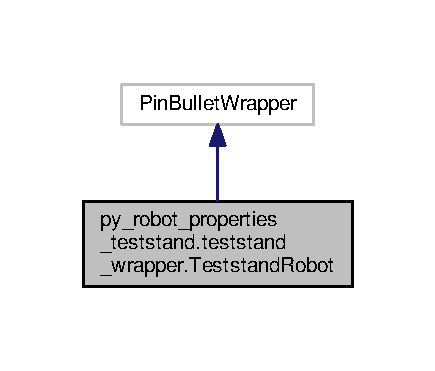
\includegraphics[width=209pt]{classpy__robot__properties__teststand_1_1teststand__wrapper_1_1TeststandRobot__inherit__graph}
\end{center}
\end{figure}


Collaboration diagram for py\+\_\+robot\+\_\+properties\+\_\+teststand.\+teststand\+\_\+wrapper.\+Teststand\+Robot\+:
\nopagebreak
\begin{figure}[H]
\begin{center}
\leavevmode
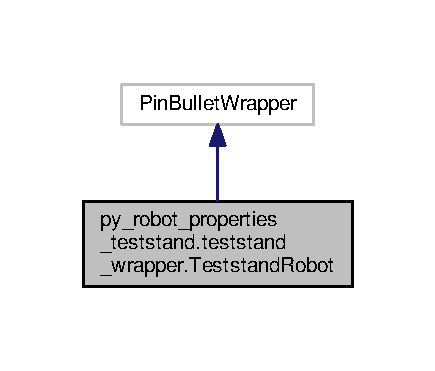
\includegraphics[width=209pt]{classpy__robot__properties__teststand_1_1teststand__wrapper_1_1TeststandRobot__coll__graph}
\end{center}
\end{figure}
\subsection*{Public Member Functions}
\begin{DoxyCompactItemize}
\item 
def {\bfseries \+\_\+\+\_\+init\+\_\+\+\_\+} (self, physics\+Client=None, fixed\+\_\+height=None)\hypertarget{classpy__robot__properties__teststand_1_1teststand__wrapper_1_1TeststandRobot_a627d6d55ef3784570f85bd3f6f683e28}{}\label{classpy__robot__properties__teststand_1_1teststand__wrapper_1_1TeststandRobot_a627d6d55ef3784570f85bd3f6f683e28}

\item 
def {\bfseries forward\+\_\+robot} (self, q=None, dq=None)\hypertarget{classpy__robot__properties__teststand_1_1teststand__wrapper_1_1TeststandRobot_aae85594daabfb7a0b44731b2dab5ce5e}{}\label{classpy__robot__properties__teststand_1_1teststand__wrapper_1_1TeststandRobot_aae85594daabfb7a0b44731b2dab5ce5e}

\end{DoxyCompactItemize}
\subsection*{Static Public Member Functions}
\begin{DoxyCompactItemize}
\item 
def {\bfseries init\+Physics\+Client} ()\hypertarget{classpy__robot__properties__teststand_1_1teststand__wrapper_1_1TeststandRobot_ab700000fd34f7e37de71798e7fdb76b7}{}\label{classpy__robot__properties__teststand_1_1teststand__wrapper_1_1TeststandRobot_ab700000fd34f7e37de71798e7fdb76b7}

\end{DoxyCompactItemize}
\subsection*{Public Attributes}
\begin{DoxyCompactItemize}
\item 
{\bfseries physics\+Client}\hypertarget{classpy__robot__properties__teststand_1_1teststand__wrapper_1_1TeststandRobot_aa4437ff4d8945c315421b5e70d3af601}{}\label{classpy__robot__properties__teststand_1_1teststand__wrapper_1_1TeststandRobot_aa4437ff4d8945c315421b5e70d3af601}

\item 
{\bfseries plane\+Id}\hypertarget{classpy__robot__properties__teststand_1_1teststand__wrapper_1_1TeststandRobot_a04fb410e4674695ce47958757348194f}{}\label{classpy__robot__properties__teststand_1_1teststand__wrapper_1_1TeststandRobot_a04fb410e4674695ce47958757348194f}

\item 
{\bfseries urdf\+\_\+path}\hypertarget{classpy__robot__properties__teststand_1_1teststand__wrapper_1_1TeststandRobot_aec6a5a48a83dca0dd1b47c7ab368ceeb}{}\label{classpy__robot__properties__teststand_1_1teststand__wrapper_1_1TeststandRobot_aec6a5a48a83dca0dd1b47c7ab368ceeb}

\item 
{\bfseries robot\+Id}\hypertarget{classpy__robot__properties__teststand_1_1teststand__wrapper_1_1TeststandRobot_a658e7fb26e593dde178f3d493fe56983}{}\label{classpy__robot__properties__teststand_1_1teststand__wrapper_1_1TeststandRobot_a658e7fb26e593dde178f3d493fe56983}

\item 
{\bfseries pin\+\_\+robot}\hypertarget{classpy__robot__properties__teststand_1_1teststand__wrapper_1_1TeststandRobot_a5a36d31d24a80328cd648b6e3fa21888}{}\label{classpy__robot__properties__teststand_1_1teststand__wrapper_1_1TeststandRobot_a5a36d31d24a80328cd648b6e3fa21888}

\item 
{\bfseries base\+\_\+link\+\_\+name}\hypertarget{classpy__robot__properties__teststand_1_1teststand__wrapper_1_1TeststandRobot_a5b1f744786d19f37a6c5d271678f3c3d}{}\label{classpy__robot__properties__teststand_1_1teststand__wrapper_1_1TeststandRobot_a5b1f744786d19f37a6c5d271678f3c3d}

\item 
{\bfseries joint\+\_\+names}\hypertarget{classpy__robot__properties__teststand_1_1teststand__wrapper_1_1TeststandRobot_a59a42e2e276864865bd7052cc8ca10b5}{}\label{classpy__robot__properties__teststand_1_1teststand__wrapper_1_1TeststandRobot_a59a42e2e276864865bd7052cc8ca10b5}

\end{DoxyCompactItemize}


The documentation for this class was generated from the following file\+:\begin{DoxyCompactItemize}
\item 
src/py\+\_\+robot\+\_\+properties\+\_\+teststand/teststand\+\_\+wrapper.\+py\end{DoxyCompactItemize}

\chapter{File Documentation}
\hypertarget{config_8py}{}\section{src/py\+\_\+robot\+\_\+properties\+\_\+teststand/config.py File Reference}
\label{config_8py}\index{src/py\+\_\+robot\+\_\+properties\+\_\+teststand/config.\+py@{src/py\+\_\+robot\+\_\+properties\+\_\+teststand/config.\+py}}


Define the interface between the control and the hardware.  


\subsection*{Classes}
\begin{DoxyCompactItemize}
\item 
class \hyperlink{classpy__robot__properties__teststand_1_1config_1_1TeststandConfig}{py\+\_\+robot\+\_\+properties\+\_\+teststand.\+config.\+Teststand\+Config}
\end{DoxyCompactItemize}


\subsection{Detailed Description}
Define the interface between the control and the hardware. 

\begin{DoxyAuthor}{Author}
Maximilien Naveau (\href{mailto:maximilien.naveau@gmail.com}{\tt maximilien.\+naveau@gmail.\+com}) 
\end{DoxyAuthor}
\begin{DoxyRefDesc}{License}
\item[\hyperlink{license__license000003}{License}]License B\+S\+D-\/3-\/\+Clause \end{DoxyRefDesc}
\begin{DoxyCopyright}{Copyright}
Copyright (c) 2019, New York University and Max Planck Gesellschaft. 
\end{DoxyCopyright}
\begin{DoxyDate}{Date}
2019-\/05-\/22 
\end{DoxyDate}

%--- End generated contents ---

% Index
\backmatter
\newpage
\phantomsection
\clearemptydoublepage
\addcontentsline{toc}{chapter}{Index}
\printindex

\end{document}
